\newcommand{\nom}{Porte conteneur}
\newcommand{\sequence}{03}
\newcommand{\num}{04}
\newcommand{\type}{TD}
\newcommand{\descrip}{Résolution d'un problème en utilisant des méthodes algorithmiques}
\newcommand{\competences}{Alt-C3: Concevoir un algorithme répondant à un problème précisément posé}
\documentclass[10pt,a4paper]{article}
  \usepackage[french]{babel}
  \usepackage[utf8]{inputenc}
  \usepackage[T1]{fontenc}
  \usepackage{xcolor}
  \usepackage[]{graphicx}
  \usepackage{makeidx}
  \usepackage{textcomp}
  \usepackage{amsmath}
  \usepackage{amssymb}
  \usepackage{stmaryrd}
  \usepackage{fancyhdr}
  \usepackage{lettrine}
  \usepackage{calc}
  \usepackage{boxedminipage}
  \usepackage[french,onelanguage, boxruled,linesnumbered]{algorithm2e}
  \usepackage[colorlinks=false,pdftex]{hyperref}
  \usepackage{minted}
  \usepackage{url}
  \usepackage[locale=FR]{siunitx}
  \usepackage{multicol}
  \usepackage{tikz}
  \makeindex

  %\graphicspath{{../Images/}}

%  \renewcommand\listingscaption{Programme}

  %\renewcommand{\thechapter}{\Alph{chapter}}
  \renewcommand{\thesection}{\Roman{section}}
  %\newcommand{\inter}{\vspace{0.5cm}%
  %\noindent }
  %\newcommand{\unite}{\ \textrm}
  \newcommand{\ud}{\mathrm{d}}
  \newcommand{\vect}{\overrightarrow}
  %\newcommand{\ch}{\mathrm{ch}} % cosinus hyperbolique
  %\newcommand{\sh}{\mathrm{sh}} % sinus hyperbolique

  \textwidth 160mm
  \textheight 250mm
  \hoffset=-1.70cm
  \voffset=-1.5cm
  \parindent=0cm

  \pagestyle{fancy}
  \fancyhead[L]{\bfseries {\large PTSI -- Dorian}}
  \fancyhead[C]{\bfseries{{\type} \no \numero}}
  \fancyhead[R]{\bfseries{\large Informatique}}
  \fancyfoot[C]{\thepage}
  \fancyfoot[L]{\footnotesize R. Costadoat, C. Darreye}
  \fancyfoot[R]{\small \today}
  
  \definecolor{bg}{rgb}{0.9,0.9,0.9}
  
  
  % macro Juliette
  
\usepackage{comment}   
\usepackage{amsthm}  
\theoremstyle{definition}
\newtheorem{exercice}{Exercice}
\newtheorem*{rappel}{Rappel}
\newtheorem*{remark}{Remarque}
\newtheorem*{defn}{Définition}
\newtheorem*{ppe}{Propriété}
\newtheorem{solution}{Solution}

\newcounter{num_quest} \setcounter{num_quest}{0}
\newcounter{num_rep} \setcounter{num_rep}{0}
\newcounter{num_cor} \setcounter{num_cor}{0}

\newcommand{\question}[1]{\refstepcounter{num_quest}\par
~\ \\ \parbox[t][][t]{0.15\linewidth}{\textbf{Question \arabic{num_quest}}}\parbox[t][][t]{0.85\linewidth}{#1\label{q\the\value{num_quest}}}\par
~\ \\}

\newcommand{\reponse}[4][1]
{\noindent
\rule{\linewidth}{.5pt}\\
\textbf{Question\ifthenelse{#1>1}{s}{} \multido{}{#1}{%
\refstepcounter{num_rep}\ref{q\the\value{num_rep}} }:} ~\ \\
\ifdef{\public}{#3 ~\ \\ \feuilleDR{#2}}{#4}
}

\newcommand{\cor}
{\refstepcounter{num_cor}
\noindent
\rule{\linewidth}{.5pt}
\textbf{Question \arabic{num_cor}:} \\
}


\usepackage{enumitem}
\usepackage{pdfpages}

\setenumerate[1]{align=left,label=\arabic*}
\setenumerate[2]{before=\stepcounter{enumi},label*=.\arabic*,leftmargin=1.2em,align=left}


\ifdef{\public}{\excludecomment{solution}}


\begin{document}

\begin{center}
{\Large\bf {\type} \no {\numero} -- \descrip}
\end{center}

\SetKw{KwFrom}{de} 

\begin{boxedminipage}{.9\textwidth} 
\begin{itemize}
 \item Faire tous les exercices dans un même fichier \textbf{NomPrenom.py} à sauvegarder,
 \item Mettre en commentaire l'exercice et la question traités (ex: \# Exercice 1),
 \item Ne pas oublier pas de commenter ce qui est fait dans votre code (ex: \# Je crée une fonction pour calculer la racine d'un nombre),
 \item Il est possible de demander un déblocage pour certaines questions, mais celle-ci seront notées 0,
 \item Il faut vérifier avant de partir que le code peut s'exécuter et qu'il affiche les résultats que vous attendez. Les lignes de code qui doivent s'exécuter sont décommentées.
\end{itemize}
\end{boxedminipage}

\section*{Présentation du thème du sujet}

Les fichiers contenant des photos possèdent des informations sur celles-­ci, elles sont communément appelées données \verb?exif?. Entre autres, on y trouve :
\begin{itemize}
\item­ la date où elle a été prise,
\item­ les coordonnées GPS de l’endroit où elle a été prise.
\end{itemize}

Le but de ce sujet est de faire un script qui va placer géographiquement sur une carte numérique les noms de fichiers photos archivés. On ajoutera des fonctionnalités à ce script au fur et à mesure de l’avancement du sujet, et la dernière partie permettra de travailler sur des informations concernant ces fichiers de photos en interrogeant une base de données. Dans tout le sujet, on supposera les modules Python importés.

\section{Géolocalisation de photos}

Le script suivant montre que deux dates sous la forme d'une chaîne de caractères peuvent être classées.

\begin{minted}{python}
x='2020:06:12 21:12:40'
y='2020:06:12 21:32:40'
print(x>y)
\end{minted}

Le script pour fonctionner devra avoir en en-tête les deux lignes suivantes:

\begin{minted}{python}
import os
os.chdir('photos')
\end{minted}

Lors des questions Q2, Q3 et Q4, les chaînes de caractères contiennent une fois et une seule le caractère \verb?'.'?.

Exemple : \verb?mot1='chat.jpg'?, mot2=\verb?'chien.jpeg'?, mot3=\verb?'fichier.ipynb'?

Les chaînes de caractères qui commencent par \verb?'.'? sont exclues.

Exemple :\verb?'.ipynb'?, \verb?'.jpg'? sont exclues.

\question{Écrire une fonction nommée \verb?placeDuPoint? qui prend en entrée une chaîne de caractères et qui retourne l’indice du point dans cette chaîne caractères.}

Exemple : dans \verb?'devoir.ipynb'? le point a pour indice 6.

\begin{solution}~\ \\
\begin{minted}{python}
def placeDuPoint(chaine):
    for i in range(len(chaine)):
        if chaine[i] == ".":
            return i

print(placeDuPoint('devoir.ipynb'))
\end{minted}
\end{solution}

\question{Écrire une fonction nommée \verb?coupeExtension? qui prend en entrée une chaîne de caractères et qui retourne la chaîne de caractères précédent le caractère '.'.}

Exemple : la fonction appliquée à \verb?'devoir.ipynb'? retourne 'devoir'.

\begin{solution}~\ \\
\begin{minted}{python}
def coupeExtension(nom_fichier):
    id_point = placeDuPoint(nom_fichier)
    return nom_fichier[:id_point]
print(coupeExtension('devoir.ipynb'))
\end{minted}
\end{solution}

\question{Écrire une fonction nommée \verb?jpgTohtml? qui prend en entrée une chaîne de caractères représentant le nom d’un fichier avec son extension et qui retourne le nom avec l’extension .html.}

Exemple : la fonction appliquée à \verb?'photo.jpg'? retourne \verb?'photo.html'?.

\begin{solution}~\ \\
\begin{minted}{python}
def jpgTohtml(nom_fichier):
    nom_sans_extension = coupeExtension(nom_fichier)
    return nom_sans_extension + ".html"
print(jpgTohtml('photo.jpg'))
\end{minted}
\end{solution}

\section{Lecture de données exif}

Dans cette partie, il est important de lire attentivement l’annexe 2 partie module exif.

On rappelle l’utilisation de la fonction \verb?openImage? :
\begin{minted}{python}
myimage=openImage("photo.jpg")
\end{minted}

La variable \verb?myimage? permet alors d’accéder aux données \verb?exif? et on fera référence à cette variable dans toute la suite du sujet.

Ainsi, il faut avant de continuer ajouter au script les lignes suivantes:
\begin{minted}{python}
from exif import Image

def openImage(nom): #nom est une chaîne de caractère qui représente ici une photo
    with open (nom, 'rb') as imageFile:
        return Image(imageFile)
myimage = openImage('photo.jpg')
\end{minted}

La question suivante se réfère à la partie Coordonnées GPS­ Règles de Conversion de l’annexe 2.

\question{Écrire une fonction \verb?convertTodecimale? qui prend en entrée un tuple (degré, minutes, secondes) et qui retourne le flottant correspondant. Vérifier le fonctionnement de la fonction en convertissant le tuple de l'annexe 2 : (36,10,11.78) grâce à un \verb?print(convertTodecimale((36,10,11.78))?.}

\begin{solution}~\ \\
\begin{minted}{python}
def convertTodecimale(angle_tuple):
    degre, minutes, secondes = angle_tuple
    return degre + 1 / 60 * minutes +  1 / 3600 * secondes 
print(convertTodecimale((36,10,11.78)))
\end{minted}
\end{solution}

On définit un type Point comme étant un tuple (latitude, longitude) de deux flottants signés.


\question{Écrire une fonction \verb?imageToGpsPoint? qui prend en entrée une variable \verb?myimage? et qui retourne une variable de type Point.}

\begin{solution}~\ \\
\begin{minted}{python}
def imageToGpsPoint(im):
    latitude = convertTodecimale(im.gps_latitude)
    if im.gps_latitude_ref == 'S':
        # la latitude est négative, on prend l'opposé
        latitude *= -1
    longitude = convertTodecimale(im.gps_longitude)
    if im.gps_longitude_ref == 'W':
        # la longitude est négative, on prend l'opposé
        longitude *= -1
    return (latitude, longitude)
print(imageToGpsPoint(my_image))
\end{minted}
\end{solution}

\question{Afficher les coordonnées GPS de toutes les photos \verb?photos0.jpg?, ..., \verb?photos7.jpg?.} 

\begin{solution}~\ \\
\begin{minted}{python}
listePhotos = ['photo{}.jpg'.format(k) for k in range(8)]

for photo in listePhotos:
    myimage = openImage(photo)
    print(imageToGpsPoint(myimage))
\end{minted}
\end{solution}

Les coordonnées du lycée Dorian, sont les suivantes:
\verb?lycee_dorian=[48.854411, 2.392279]?.

\question{Écrire une fonction \verb?calculDistance(point1,point2)? qui prend en entrée deux points définis par leur coordonnées (latitude, longitude) et qui donne la distance relative définie comme la norme du vecteur entre ces deux points.}

Ainsi, la distance entre le lycée Dorian et les coordonnées GPS de la photo \verb?photo0.jpg}? est 9.22267829505805 (attention, ce n'est pas une distance en mètre).

\begin{solution}~\ \\
\begin{minted}{python}
lycee_dorian=[48.854411, 2.392279]

def calculDistance(point1,point2):
    return ((point1[0]-point2[0])**2+(point1[1]-point2[1])**2)**(1/2)
myimage = openImage('photo0.jpg')
print(calculDistance(imageToGpsPoint(my_image),lycee_dorian)])
\end{minted}
\end{solution}

\question{Générer une liste \verb?distances? contenant l'ensemble des couples \verb?['nomphoto',distance]? dont la distance correspond à celle entre l'endroit où la photo a été prise et le lycée Dorian. Afficher \verb?distances[0]?.}

Le résultats de l'instruction \verb?print(distances[0])? doit être \verb?['photo0.jpg', 9.22267829505805]?.

\begin{solution}~\ \\
\begin{minted}{python}
distances=[]

for photo in listePhotos:
    my_image = openImage(photo)
    distances.append([photo,calculDistance(imageToGpsPoint(myimage),lycee_dorian)])

print(distances[0])   
\end{minted}
\end{solution}

\question{A l'aide d'une fonction de tri de votre choix, classer la liste \verb?distances? de la distance la plus petite à la plus grande. Afficher la liste \verb?distances? ainsi triée.}

\begin{solution}~\ \\
\begin{minted}{python}
def tri_bulle(liste):
    # Parcours de 1 à la taille de la liste
    for i in range(1, len(liste)):
        # Parcours des éléments précédents
        for j in range(0, len(liste)-i):
            # On permutte les deux éléments successifs
            if liste[j][1] > liste[j+1][1] :
                liste[j], liste[j+1] = liste[j+1], liste[j]

tri_bulle(distances)
print(distances)
\end{minted}
\end{solution}

\question{Afficher les noms et les distances de la photo la plus proche et de la plus éloignée.}

\begin{solution}~\ \\
\begin{minted}{python}
print('La photo prise la plus près est la {}.'.format(coupeExtension(distances[0][0])))
print('La photo prise la plus loin est la {}.'.format(coupeExtension(distances[-1][0])))
\end{minted}
\end{solution}

\question{Écrire une fonction \verb?listeApresGouter? qui prend en entrée une liste de photos (les photos sont représentées par leur nom qui est une chaîne de caractères) et qui retourne la liste des photos prises après 17h.}

\begin{solution}~\ \\
\begin{minted}{python}
def listeApresGouter(photos):
    avant_midi = []
    for photo in photos:
        my_image = openImage(photo)
        var_date = my_image.datetime
        heure = var_date[11:13]
        if heure > "17":
            avant_midi.append(photo)
    return avant_midi

print(listeApresGouter(listePhotos))
\end{minted}
\end{solution}

\section{Recherche des dossiers des photos}

Dans le but de rechercher des photos dans un dossier, nous allons commencer par rechercher tous les dossiers dans un dossier principal \verb?Arborescence?.

Pour continuer, il faudra copier le code suivant dans le script.

\begin{minted}{python}
def listAbsolutePath(directory):
    for dirpath,dirs,filenames in os.walk(directory):
        return sorted([os.path.abspath(os.path.join(dirpath, d)) for d in dirs])

os.chdir('Arboresence')

s=listAbsolutePath('Arboresence')[0]
print(s)
\end{minted}

Il permet de créer la fonction \verb?listAbsolutePath(directory)? qui permet de lister les sous-dossiers contenus dans le dossier \verb?directory?. 

~\

On rappelle donne dans la suite une méthode permettant le parcours du graphe \verb?gr? en largeur.

\begin{minted}{python}
gr={'A':['B','D','E'],'B':['A','C','E'],'C':['B','D'],'D':['A','C'],'E':['A','B']}

def parcoursLargeur(gr,s):
    files=[s]
    noeuds_decouverts=[s]
    while len(files)!=0:
        noeud_courant=files[0]
        files=files[1:]
        for voisin in gr[noeud_courant]:
            if voisin not in noeuds_decouverts:
                noeuds_decouverts.append(voisin)
                files.append(voisin)
    return(noeuds_decouverts)

print(parcoursLargeur(gr,'A'))
\end{minted}

\question{Adapter cette méthode en utilisant la fonction \verb?listAbsolutePath(directory)? afin de lister l'ensemble des sous-dossiers du dossier \verb?Arborescence?. Stocker l'ensemble de ces éléments dans une liste \verb?noeudsDecouverts?.}

\begin{solution}~\ \\
\begin{minted}{python}
files=[s]
noeudsDecouverts=[s]
while len(files)!=0:
    noeud_courant=files[0]
    files=files[1:] 
    for voisin in listAbsolutePath(noeud_courant):
        if voisin not in noeuds_decouverts:
            noeudsDecouverts.append(voisin)
            files.append(voisin)
print(noeudsDecouverts)
\end{minted}
\end{solution}

Dans cette dernière partie, nous souhaitons récupérer simplement les noms des dossiers sans leur chemin absolu.

\question{Proposer une solution permettant de créer une chaîne de caractères contenant les noms des dossiers seuls sans leur chemin relatif, dans leur ordre d'apparition par le parcours en largeur. Vous pourrez utiliser la fonction \verb?split?.}

\begin{solution}~\ \\
\begin{minted}{python}
chaine=''
for dir in noeuds_decouverts:
    chaine+=dir.split('/')[-1]
print(chaine)
\end{minted}
\end{solution}

\newpage

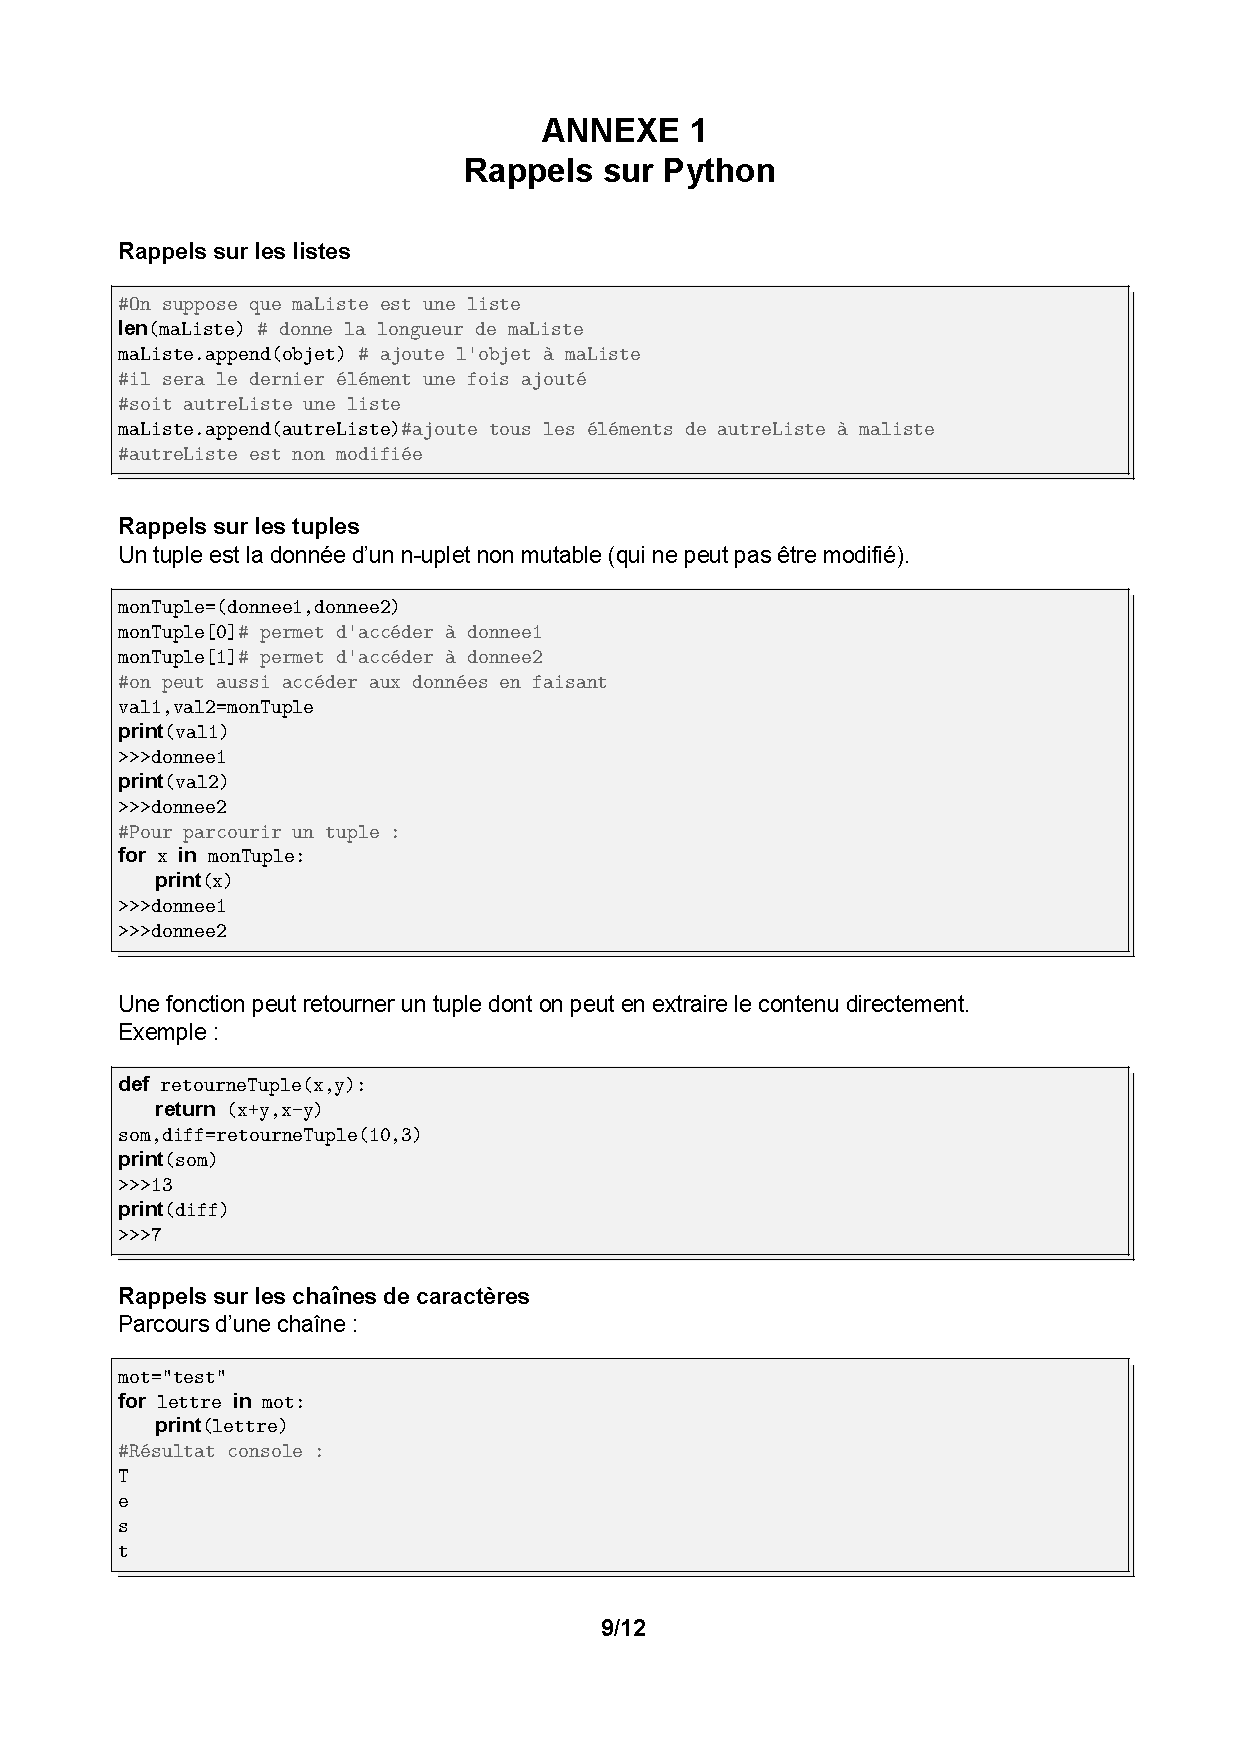
\includepdf[pages=1-3,offset=50 -50]{annexes.pdf}

\end{document}




